É um fenómeno de troca de energia que ocorre naturalmente onde o fluxo de energia percorre um corpo de maior temperatura para um corpo de menor temperatura até que ambos atinjam o equilíbrio térmico. 

\begin{enumerate}
\item \textbf{Condução}\\ 
Na condução existem duas superfícies em contato que devido ao gradiente de temperatura promovem o equilíbrio térmico sem que haja troca de matéria entre estas superfícies.

Temos a \emph{Lei de Fourier} que nos dá a taxa de transferência de
calor através de uma superfície S é proporcional à sua área e ao gradiente de temperatura sobre a mesma, dada pela equação:

\[\frac{dQ}{dt}=-k A \frac{dT}{dx}\] \\

$ \frac{dQ}{dt} $ é o gradiente de temperatura na direção perpendicular à superfície dado em K/m.

Quando utilizamos as propriedades de condutância e resistência térmica dos materiais, temos a seguinte equação para \emph{Lei de Fourier}:

\[\frac{dQ}{dt}=-U \Delta T = -\frac{\Delta T}{R}\] \\

onde \emph{U} é a condutância do material e \emph{R} é a resistência.
\item \textbf{Convecção} \\
Convecção é a transferência de calor devido ao deslocamento da matéria, mais especificamente, o movimento de fluidos.
Este fenómeno será estudado aqui pois teremos o \emph{heatsink} ( dissipador de calor ) que vem a ser regido por essa condição de troca de calor.
 \begin{itemize}
 \item \textit{Convecção natural:} Quando o deslocamento do fluido é causado pelo empuxo resultante
de uma diferença de densidade, causada por variações na temperatura do
fluido.
\item \textit{Convecção forçada:} Quando o fluido é forçado a se deslocar por um dispositivo
externo como um ventilador ou bomba.
 \end{itemize}
 Assim temos que pela \emph{lei de Newton} para o resfriamento diz que a taxa de transferência de calor de
um corpo, devido à convecção, é proporcional à diferença de temperatura entre o corpo e
o ambiente e à sua área de contato.

\[\frac{dQ}{dt}= h A \Delta T\] \\

Onde:\\
$ \frac{dQ}{dt} $ é o fluxo de calor em Watts, ou seja, a quantidade de calor por unidade de tempo que deixa o corpo;\\
\emph{h} é o coeficiente de transferência térmica dado em $ W/m^{2} K $; \\
$ \Delta T $ é a diferença entre a temperatura do corpo e a temperatura ambiente K.\\
\item \textbf{Efeito Termoelétrico }\\
É o efeito gerado através da aplicação de uma diferença de potencial elétrico em um elemento de circuito que converte diretamente em uma diferença de temperatura neste elemento e vice-versa. \\
Portanto, dispositivos termo-elétricos podem ser utilizados para gerar eletricidade, medir temperatura, aquecer ou resfriar objetos.
Em nosso projeto faremos uso destes elementos de circuito para deles obter 3 dos principais efeitos termo-elétricos:

\begin{itemize}
\item \textbf{\emph{O efeito Seebeck}} \cite{huang2000system}, descoberto pelo físico Estoniano Thomas Johann Seebeck;\\
O efeito de Seebeck é o princípio de operação dos termopares, dispositivos utilizados para medir temperatura. \\
Pode ser calculado por:
\[V=\left ( S_{A}-S_{B} \right )\left ( T_{2}-T_{1} \right )\] \\

\item \textbf{\emph{O efeito Peltier}} \cite{huang2000system}, descoberto pelo físico Frances Jean Charles Athanase Peltier;\\
O efeito peltier é o princípio de operação dos dispositivos de refrigeração termo-elétricos. Esse efeito pode ser calculado por:\\
\[\frac{dQ}{dt}=\left ( \Pi_{B} -\Pi _{A} \right )\ast I\] \\

Onde:\\
$ \Pi _{A} e \Pi _{B} $ são os coeficientes de Peltier para os materiais A e B respectivamente e dependem da temperatura da Junção. Nota-se que se $ \Pi _{A} > \Pi _{B} $ há geração de calor,
caso contrário há absorção de calor.


\item \textbf{\emph{O efeito Thomson}} \cite{huang2000system}, descoberto pelo físico Britânico William Thomson (Lord Kelvin). \\


\end{itemize}
Cada um destes efeitos, são utilizados em sensores de temperatura atuadores de resfriamento e/ou aquecimento, em cada um deles será feito o devido tratamento matemático afim de se obter sua respectiva \emph{Equação de Estado}.\\
Estes efeitos se relacionam com portadores de difusão de cargas em circuitos semicondutores. 

\item \textbf{Modulo Peltier} \\
Módulos de peltier são dispositivos que utilizam o efeito Peltier para transferir calor de um lado frio para um lado quente com a aplicação de uma corrente em seus terminais.
São frequentemente utilizados para o resfriamento de dispositivos eletrônicos como CPUs, sensores de infravermelho, manutenção de temperaturas de referência em termopares e refrigeradores.
A eficiência de um módulo de peltier depende da quantidade de calor transferida, da diferença de temperatura entre seus lados e da corrente aplicada. Um módulo de Peltier típico é composto de junções tipo P e N do semicondutor Teluro de Bismuto com um metal M como na figura.\\
	
Duas junções tipo P e N formam o que se denomina uma junção ou par. O módulo possui várias junções conectadas eletricamente em série 4.\\
Os semicondutores tipo \emph{P} e \emph{N} e o metal \emph{M} são tais que seus coeficientes de Seebeck obedecem:\\
\[\alpha _{N}> \alpha _{M}> \alpha _{P}\]\\
Quando a corrente I atravessa cada junção da figura \ref{fig:Ppeltier}, o calor é absorvido nas junções P-M e M-N e produzido nas junções M-P e N-M.\\
\begin{minipage}{0.5\linewidth}
Deste modo, cria-se uma região de absorção de calor (topo) e produção de calor (base). Várias junções são dispostas termicamente em paralelo para amplificar este efeito.
O módulo de peltier típico usa também duas pastilhas cerâmicas finas em ambos os lados que fornecem a isolação elétrica e a rigidez mecânica necessária.
\end{minipage}
\begin{minipage}{0.5\linewidth}
\begin{figure}[H]
		\centering
		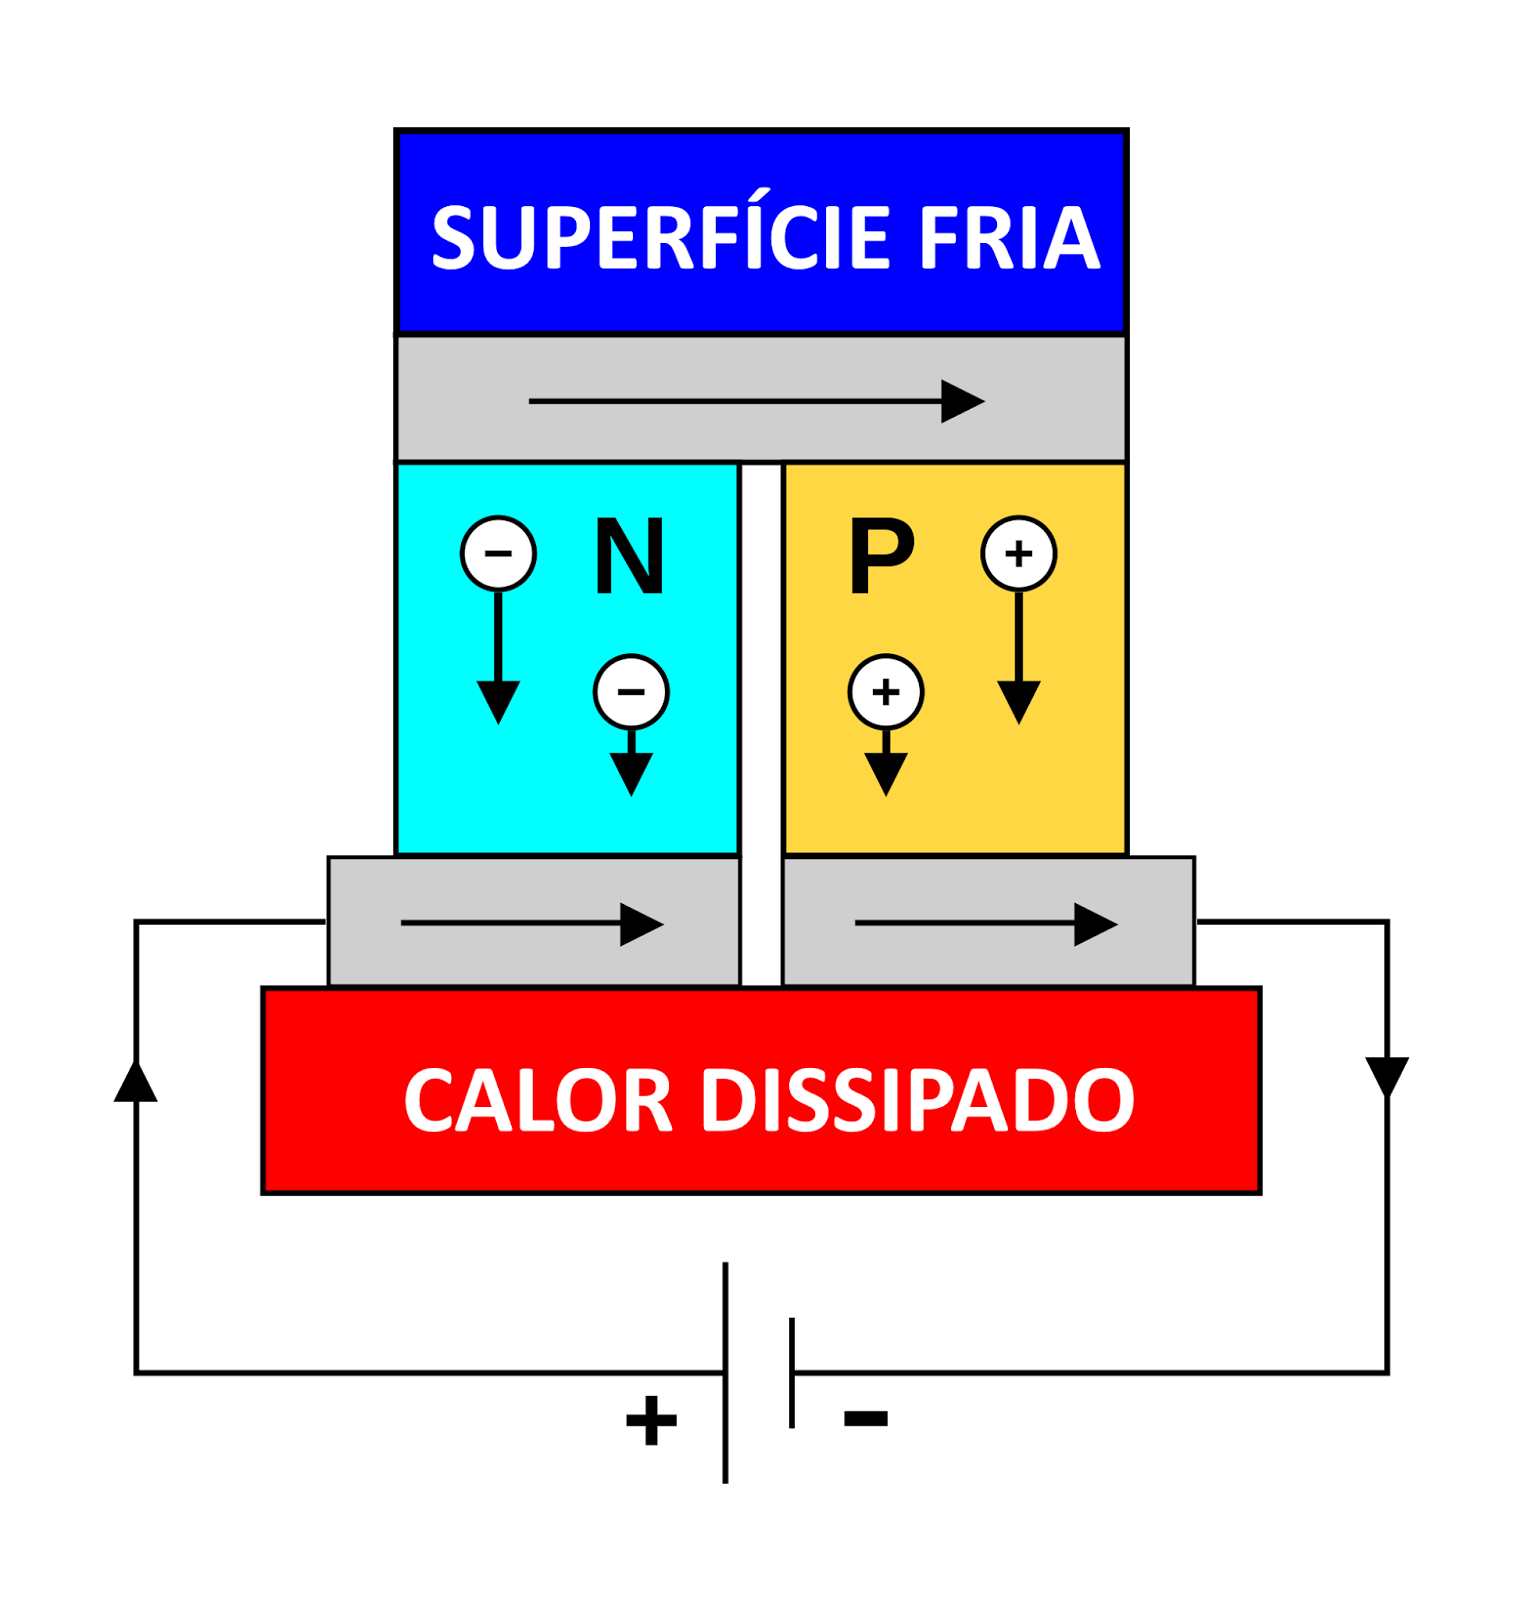
\includegraphics[width=0.7\linewidth]{./ima/peltier02.jpg}
		\label{fig:Ppeltier}
		\caption{Esquema Pastilha Peltier}
	\end{figure}
\end{minipage}



\end{enumerate}
